
\section{Case Study}\label{sec:imp_cs}
To show the efficacy of our approach in transforming and using produced AADL models to analyze the properties, this section presents the experimental results of analyzing the traction controlling unit of railway signaling system. By using our proposed approach, we transfer and extend Arcadia metamodel, and design AADL using OSATE2~\cite{osate2ref} with the generated metamodel. once the concrete models have been created, the scheduling property is chosen to show analysis ability through Cheddar tool. 



\subsection{Train traction controlling system (TCU)}
Train movement is the calculation of the speed and distance profiles when a train is traveling from one point to another according to the limitations imposed by the signaling system and traction equipment characteristics. As the train has to follow the track, the movement is also under the constraints of track geometry, and speed restrictions and the calculation becomes position-dependent. The subsystem of calculating the traction effective and speed restrictions is therefore critical to achieving train safe running.
Nowadays, Communication based train control (CBTC) is the main method of rail transit (both urban and high-speed train) which adopts wireless local area networks as the bidirectional train-ground communication~\cite{zhu2009train}. To increase the capacity of rail transit lines, many information-based and digital components have been applied for networking, automation and system inter-connection, including general communication technologies, sensor networks, and safety-critical embedded control system. %A large number of subsystems consisting of modern signaling systems of railways, therefore, system integration is one of the key technologies of signaling systems; it plays a significant role in maintaining the safety of the signaling system~\cite{Wang:gg}. 

This paper uses a subsystem called traction controlling system (TCU) from signalling system of high-speed railways to illustrate the model transformation from engineering level to detailed architectural level and verification of instance models. Functional modules such as calculation and synchronization will be transformed using our approach, and then non-functional properties such as timing correctness and resource correctness will be verified by simulation tool Cheddar~\cite{Singhoff:2004es}. 

The functions of the traction control system are to collect the external data by sensors such as speed sensor. The data from Balise sensors is used to determinate the track block, and then it is going to seek the speed restriction conditions by matching accurate positioning (if the track blocks are divided fine enough) and digital geometric maps data. Meanwhile, calculating speed unit received the speed data from GPS and speed control commands from HMI (Human-Machine Interface) periodically. GPS data provides speed value periodically, and HMI data send the operation command (e.g., expected speed value), then the calculating unit has to output an acceleration value and export to the locomotive mechanical system. Although they are periodic, the external data do not always arrive on time due to transmission delay or jitter. Therefore, we should use a synchronizer to make sure they are synchronized. Otherwise, the result would be wrong with asynchronous data. Similarly, to ensure the correctness of the command of acceleration (or deceleration), we applied a voting mechanism which can ensure the result is correct as much as possible. The voter must have the synchronized signal and restriction condition to dedicate to output the acceleration coefficient request to the locomotive system. The AADL diagram shown as figure \ref{fig:tcus}.     

\begin{figure*}[!h]
\centering
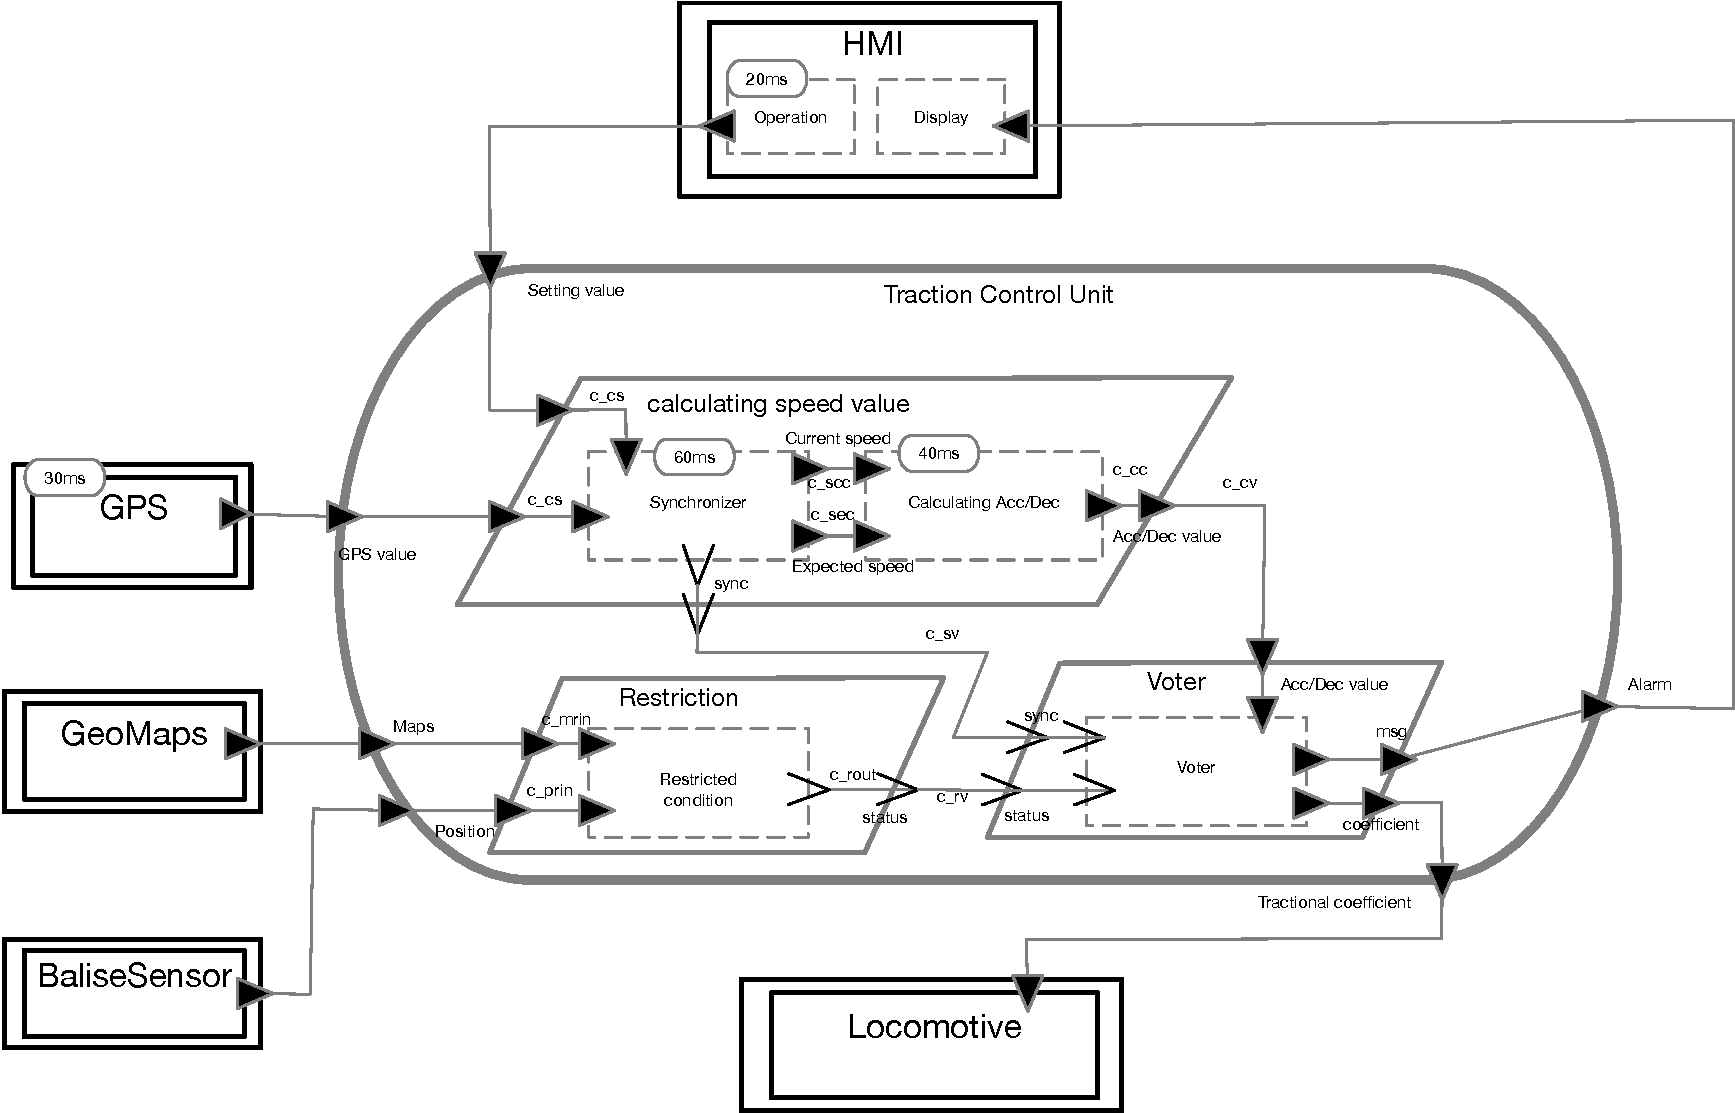
\includegraphics[width=.75\linewidth]{img/TCU_all}
\caption{AADL model for TCU of signaling system}
\label{fig:tcus}
\end{figure*}




\subsection{Model transformation}
Using the Arcadia2AADL tool, the metamodel of the TCU system in Capella is translated into the corresponding AADL metamodel with the rules and approach which describes in section \ref{sec:trans}. For instance, on the one hand, the function class is translated into the thread in AADL. To analyze the timing properties, several attributes also have been added such as protocol type, deadline, execution time, period. 

On the other hand, the physical part element Node translates to the processor in this case. Differ from simple physical Node in Arcadia; the processor element attaches rich properties such as scheduling protocol (scheduler type), process execution time. 
The allocation relationships on both physical and functional parts are translated into AADL as well.
\subsection{Schedule verification}
The external data and internal process work sequentially is an essential safety requirement of the system, and each task should be scheduled properly. However, in real-world, the risk of communication quality and rationality of scheduling must be taken into account. Therefore, the schedule verification is a way to evaluate system timing property. An Ada framework called Cheddar which provides tools to check if a real-time application meets its temporal constraints. The framework is based on the real-time scheduling theory and is mostly written for educational purposes~\cite{Singhoff:2005:SMR:1103846.1103847}.

\input{codes/cal.aadl}

Listing \ref{code:cal} shows a set of 4 periodic tasks (cal, pos, sync and setting) of TCU  respectively defined by the periods 100, 100, 40 and 30, the capacities 60, 40, 30 and 20, and the deadlines 100, 100, 40 and 30. These tasks are scheduled with a preemptive Rate Monotonic scheduler (the task with the lowest period is the task with the highest priority).
\begin{figure*}[h]
\centering
\subfigure[Schedule 1]{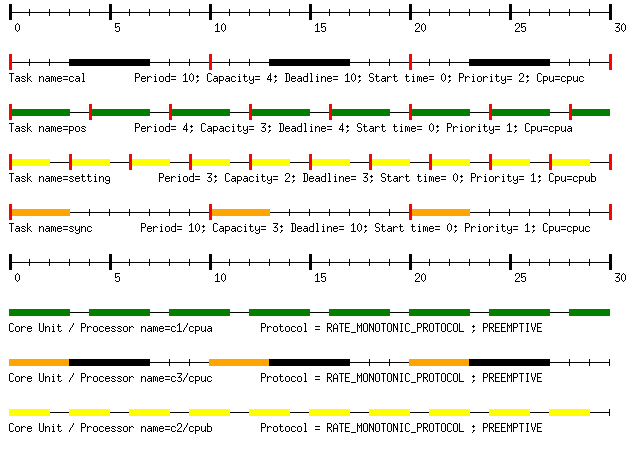
\includegraphics[width=.45\linewidth]{img/sim_left}}
\subfigure[Schedule 2]{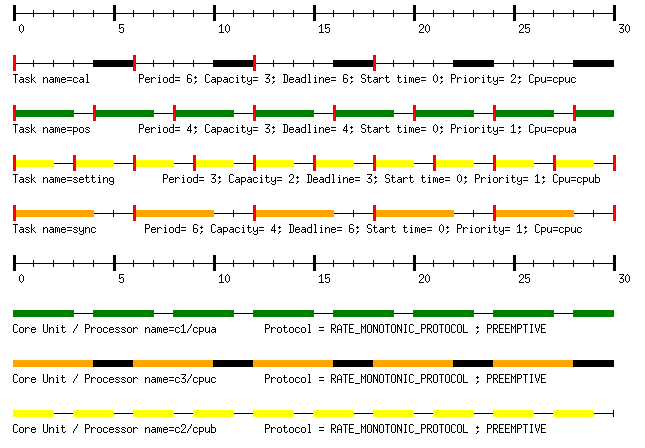
\includegraphics[width=.45\linewidth]{img/sim_right}}
\caption{Simulation results of tasks schedule}
\label{fig:sim}
\end{figure*}
For a given task set, if a scheduling simulation displayed XML results in the Cheddar. One can find the concurrency cases or idle periods (see left of figure \ref{fig:sim}, comprise the software part and physical device part). People change the parameters directly and reload simulation; an feasible solution can be applied instead. After tuning, finally, the appropriate setting has displayed as in right of figure \ref{fig:sim}. According to this simulation result, people can correct the properties value in AADL, thereby ensure the correctness of system behavior timing properties.  




%% Preamble: \pgfplotsset{width=7cm,compat=1.15} 
%\pgfplotsset{every axis/.append style={
%    font=\footnotesize,
%    thin,
%    tick style={ultra thin}},
%}
%\begin{figure}
%\begin{tikzpicture}
%    \begin{axis}[legend pos=outer north east,
%        xlabel=Time (second),
%        ylabel=Speed (km/h),
%    ]
%        \addplot+ table {codes/dataset};
%        \addplot+ table {codes/dataset1};
%        \addplot+ table {codes/dataset2};
%        \legend{caculated speed, current speed, setting speed}
%    \end{axis}
%\end{tikzpicture}
%	\caption{Train speeds}
%	\label{fig:speed}
%\end{figure}